\documentclass{beamer}
\usepackage{amsmath,amsbsy,amsopn,amstext,amsfonts,amssymb}
\usepackage{isomath}
\usepackage{ulem}
%\linespread{1.6}  % double spaces lines
\usepackage{graphicx}
\usepackage{subfigure}
\usepackage{color}
\usepackage{optidef}  % define optimization problems
\usepackage{multicol}  % multiple columns
\usepackage{listings} % for python code
\usepackage{mathrsfs}

\usepackage{polynom}
\newcommand{\adj}{\mathrm{adj}}
\newcommand{\constrainedmin}[3]{
		\begin{mini*}|s|
		{#2}{#1}{}{}
		\addConstraint{#3}
		\end{mini*}
}

\newcommand{\rwbcomment}[1]{{\color{blue}RWB:#1}}
\newcommand{\defeq}{\stackrel{\triangle}{=}}
\newcommand{\abs}[1]{\left|#1\right|}
\newcommand{\norm}[1]{\left\|#1\right\|}
\newcommand{\iprod}[1]{\left<#1\right>}
\newcommand{\ellbf}{\boldsymbol{\ell}}
\newcommand{\nubf}{\boldsymbol{\nu}}
\newcommand{\mubf}{\boldsymbol{\mu}}
\newcommand{\abf}{\mathbf{a}}
\newcommand{\bbf}{\mathbf{b}}
\newcommand{\cbf}{\mathbf{c}}
\newcommand{\dbf}{\mathbf{d}}
\newcommand{\ebf}{\mathbf{e}}
\newcommand{\fbf}{\mathbf{f}}
\newcommand{\gbf}{\mathbf{g}}
\newcommand{\hbf}{\mathbf{h}}
\newcommand{\ibf}{\mathbf{i}}
\newcommand{\jbf}{\mathbf{j}}
\newcommand{\kbf}{\mathbf{k}}
\newcommand{\lbf}{\mathbf{l}}
\newcommand{\mbf}{\mathbf{m}}
\newcommand{\nbf}{\mathbf{n}}
\newcommand{\obf}{\mathbf{o}}
\newcommand{\pbf}{\mathbf{p}}
\newcommand{\qbf}{\mathbf{q}}
\newcommand{\rbf}{\mathbf{r}}
\newcommand{\sbf}{\mathbf{s}}
\newcommand{\tbf}{\mathbf{t}}
\newcommand{\ubf}{\mathbf{u}}
\newcommand{\vbf}{\mathbf{v}}
\newcommand{\wbf}{\mathbf{w}}
\newcommand{\xbf}{\mathbf{x}}
\newcommand{\ybf}{\mathbf{y}}
\newcommand{\zbf}{\mathbf{z}}
\newcommand{\Jbf}{\mathbf{J}}
\newcommand{\Acal}{\mathcal{A}}
\newcommand{\Bcal}{\mathcal{B}}
\newcommand{\Lcal}{\mathcal{L}}
\newcommand{\Ncal}{\mathcal{N}}
\newcommand{\Rcal}{\mathcal{R}}
\definecolor{darkolivegreen}{rgb}{0.33, 0.42, 0.18}

\makeatletter
\newenvironment<>{proofstart}[1][\proofname]{%
    \par
    \def\insertproofname{#1\@addpunct{.}}%
    \usebeamertemplate{proof begin}#2}
  {\usebeamertemplate{proof end}}
\newenvironment<>{proofcont}{%
  \setbeamertemplate{proof begin}{\begin{block}{}}
    \par
    \usebeamertemplate{proof begin}}
  {\usebeamertemplate{proof end}}
\newenvironment<>{proofend}{%
    \par
    \pushQED{\qed}
    \setbeamertemplate{proof begin}{\begin{block}{}}
    \usebeamertemplate{proof begin}}
  {\popQED\usebeamertemplate{proof end}}
\makeatother

\title{ECEn 671: Mathematics of Signals and Systems}
\author{Randal W. Beard}
\institute{Brigham Young University}
\date{\today}

\begin{document}

%-------------------------------
\begin{frame}
	\titlepage
\end{frame}


%%%%%%%%%%%%%%%%%%%%%%%%%%%%%%%%%%%%%%%%%%%%%%%%%%%%%%%%%%%%%%%%%
\section{Constrained Optimization}
\frame{\sectionpage}


%----------------------------------
\begin{frame}\frametitle{Constrained Optimization}
	In Chapter 14 we studied unconstrained minimization of continuously differentiable functions.
	
	\vfill
	
	In Chapter 18 we focus on constrained optimization problems.
	
	\vfill
	
	For example, given the level curves,
	\begin{center}
		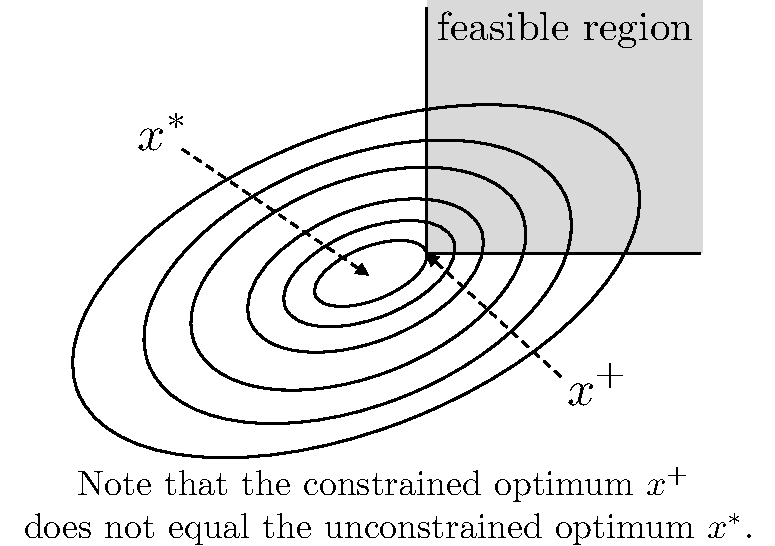
\includegraphics[width=0.5\textwidth]
			{figures/chap18_constrained_optimum}
	\end{center}
	The unconstrained optimum is $x^{\ast}$; the constained optimum is $x^{+}$.
\end{frame}

%----------------------------------
\begin{frame}\frametitle{Constrained Optimization}
	\begin{definition}
		Let $\Omega \subseteq \mathbb{R}^n$ be the feasible region.  
		Then $x^{\ast}\in \Omega$ is a \underline{local minimum} of $f:\mathbb{R}^n\to\mathbb{R}$ over $\Omega$ if $\exists \epsilon > 0$ such that 
		\[
			x \in \Omega \cap \{y\in \mathbb{R}^n:|u-x^{\ast}|<\epsilon\} \quad \implies \quad f(x) \geq f(x^{\ast}).
		\]
		If $f(x) > f(x^{\ast})$ then $x^{\ast}$ is a \underline{strict local minimum}.  
		If true for all $\epsilon > 0$ then $x^{\ast}$ is a global minimum.
	\end{definition}
	
	\vfill

	\begin{center}
		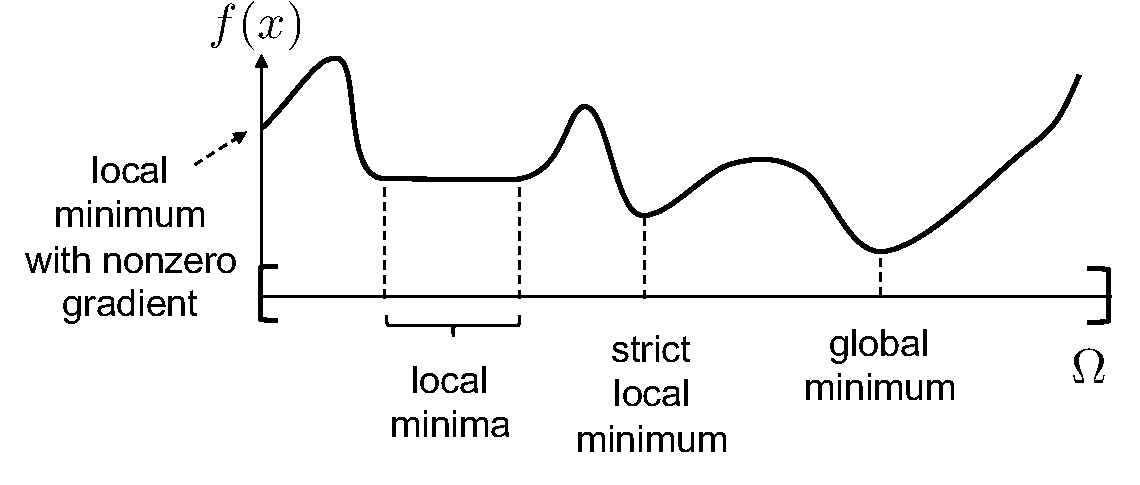
\includegraphics[width=0.6\textwidth]
			{figures/chap18_types_of_minima}
	\end{center}
\end{frame}

%----------------------------------
\begin{frame}\frametitle{Constrained Optimization}
	\begin{definition}
		Let $x \in \Omega$ and $d \in \mathbb{R}^n$, then 
		\[
			y = x+ \alpha d
		\]
		is a \underline{feasible point} if $y \in \Omega$.
	\end{definition}
	
	\vspace{0.5cm}
	
	\begin{definition}
		The vector $d$ is a \underline{feasible direction} at $x$, if $\exists\epsilon_0 > 0$ such that 
		\[
			x + \epsilon d \in \Omega
		\]		
		for every $0 \leq \epsilon \leq \epsilon_0$.
	\end{definition}
\end{frame}

%----------------------------------
\begin{frame}\frametitle{Constrained Optimization}
	Recall, if $f: \mathbb{R}^n\to\mathbb{R}$ then the gradient vector is
	\[
		\frac{\partial f}{\partial x} 
			= \nabla_x f 
			= \begin{pmatrix}
	    		\frac{\partial f}{\partial x_1}\\
	    		\vdots\\
	    		\frac{\partial f}{\partial x_n}
	  		  \end{pmatrix}
	\]
	and the Hessian matrix is
	\[ 
		\frac{\partial^2 f}{\partial x^2} 
			= \nabla^2f 
			= \begin{pmatrix}
	    		\frac{\partial^2 f}{\partial x_1^2} & \frac{\partial^2 f}{\partial x_1 \partial x_2} & \cdots & \frac{\partial^2 f}{\partial x_1 \partial x_n}\\
	    		\vdots & & & \vdots\\
	    		\frac{\partial^2 f}{\partial x_n \partial x_1} & \cdots & \cdots & \frac{\partial^2 f}{\partial x_n^2}
	  		  \end{pmatrix}.
	\]	
	If $\Omega = \mathbb{R}^n$ then a necessary condition for $x^{\ast}$ to be a local minima is that $\nabla_xf(x^{\ast})=0$.  What about constrained optimization problems?
\end{frame}

%----------------------------------
\begin{frame}\frametitle{Constrained Optimization}
	\begin{theorem}[Moon Theorem 18.1]
		Let $\Omega \subseteq \mathbb{R}^n$ and let $f:\mathbb{R}^n\to\mathbb{R}$ be $\mathcal{C}^1$ (continuously differentiable) on $\Omega$.
		
		\begin{enumerate}
		\item If $x^{\ast}$ is a local minimum of $f$ over $\Omega$, then for \underline{any} feasible direction $d \in \mathbb{R}^n$ at $x^{\ast}$
			\[ 
				\left[ \nabla_xf(x^{\ast}) \right]^\top d \geq 0 
			\]
		\item If $x^{\ast}$ is an interior point of $\Omega$, then 
			\[ 
				\nabla f(x^{\ast}) = 0.
			\]
		\item If in addition, $f \in \mathcal{C}^2$ and $\nabla_x f(x^{\ast})^\top d = 0$, then 
			\[ 
				d^\top \nabla^2f(x^{\ast})d \geq 0 
			\]
			Note that this is a weaker condition than psd Hessian.
		\end{enumerate}		
	\end{theorem}
\end{frame}

%----------------------------------
\begin{frame}\frametitle{Proof of Theorem 18.1}
	1. By Taylor series expansion,
	\begin{align*}
		& f(x^{\ast} + \epsilon d) = f(x^{\ast}) + \epsilon\nabla_xf(x^{\ast})^\top d+ O(\epsilon) \\
		\implies & f(x^{\ast}+\epsilon d) - f(x^{\ast}) = \epsilon\nabla_xf(x^{\ast})^\top d + O(\epsilon) 
	\end{align*}
	Since $x^{\ast}$ is a local minimum, for $\epsilon$ sufficiently small we must have that
	\begin{align*}
		\implies & f(x^{\ast} + \epsilon d) - f(x^{\ast}) \geq 0 \\
		\implies & \nabla_xf(x^{\ast})^\top d \geq 0.
	\end{align*}	
\end{frame}

%----------------------------------
\begin{frame}\frametitle{Proof of Theorem 18.1, cont.}
	2.  If $x^{\ast}$ is an interior point then every $d \in \mathbb{R}^n$ is feasible at $x^{\ast}$, i.e.
	\[ 
		\iprod{\nabla_xf(x^{\ast}), d }_{\mathbb{R}^n} = 0, \qquad \forall d\in\mathbb{R}^n. 
	\]
	Therefore,
	\begin{align*}
	  & \nabla_xf(x^{\ast})^\top d \geq 0 
	  	\quad \text{and} \quad 
	  	\nabla_xf(x^{\ast})^\top (-d) \geq 0\\
	  \implies & \nabla_xf(x^{\ast})^\top d = 0, \quad \forall d\in\mathbb{R}^n \\
	  \implies &  \nabla_xf(x^{\ast}) = 0
	\end{align*}
	since $R^n$ is a finite dimensional vector space	.
\end{frame}

%----------------------------------
\begin{frame}\frametitle{Proof of Theorem 18.1, cont.}
	3.  If $\nabla_xf(x^{\ast})^\top d = 0$ then the Taylor series for $f$ is
	\begin{align*}
		& f(x^{\ast}+\epsilon d) = f(x^{\ast}) + \epsilon^2d^\top \nabla^2f(x^{\ast})d + O(\epsilon^2) \\
		\implies &  0 \leq f(x^{\ast} + \epsilon d) - f(x^{\ast}) = \epsilon^2d^\top \nabla^2f(x^{\ast})d + O(\epsilon^2) \\
		\implies & d^\top \nabla^2f(x^{\ast})d \geq 0.
	\end{align*}
	\begin{center}
		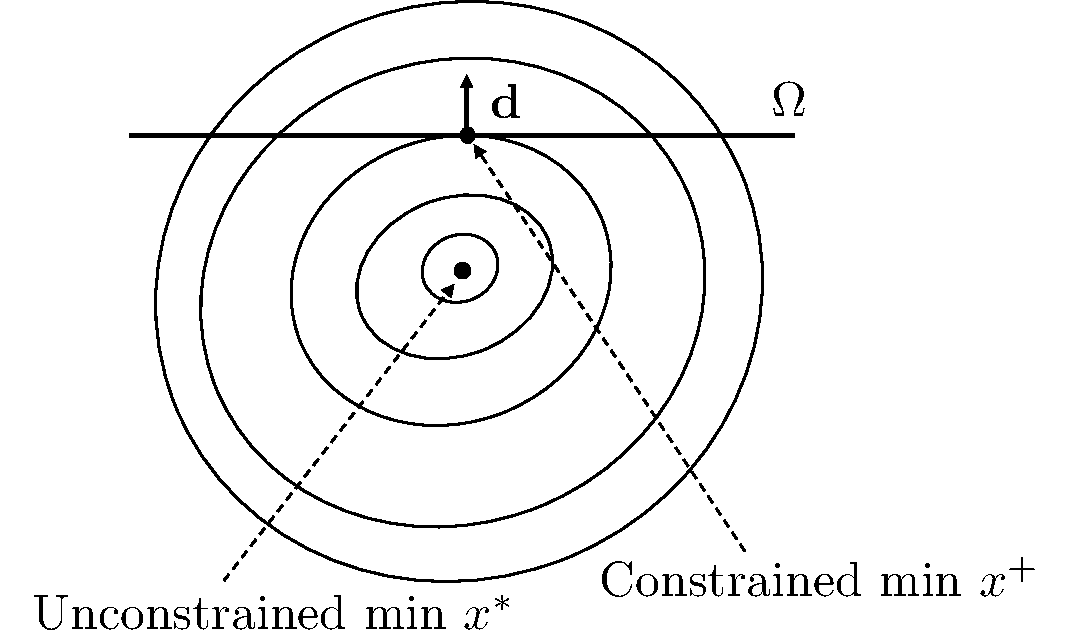
\includegraphics[width=0.5\textwidth]
			{figures/chap18_linear_constraint}
	\end{center}

	Note:  Any feasible $d$ points uphill.
	
	Note:  The function is concave in feasible region.
\end{frame}

%----------------------------------
\begin{frame}\frametitle{Constrained Optimization: Sufficient Conditions}
	\underline{Are there sufficient conditions?}
	
	\vfill
	
	First, suppose that the constraints are not active, i.e. $x^{\ast}$ is an interior point of $\Omega$.  (We will consider the active constraint case later.)
	
	\vfill
	
	\begin{theorem}[Moon Theorem 18.2]
		Let $f \in \mathcal{C}^2$ on $\Omega$ and let $x^{\ast}$ be an interior point of $\Omega$.  If $\nabla f(x^{\ast}) = 0$ and $\nabla^2f(x^{\ast})$ is positive definite then $x^{\ast}$ is a strict local minimum of $f$.
	\end{theorem}
\end{frame}

%----------------------------------
\begin{frame}\frametitle{Constrained Optimization: Sufficient Conditions: Proof}
	\begin{proof}
		Let $d$ be any unit vector in $\mathbb{R}^n$ then 
		\begin{align*}
			& 	f(x^{\ast} + \epsilon d) = f(x^{\ast}) + \epsilon\nabla f(x^{\ast})^\top d + \epsilon^2d^\top \nabla^2f(x^{\ast})d + O(\epsilon^2) \\
			\implies & 
			f(x^{\ast} + \epsilon d)  - f(x^{\ast}) = \epsilon^2d^\top \nabla^2f(x^{\ast})d + O(\epsilon^2)
		\end{align*}
	
		Since $\nabla^2f(x^{\ast})$ is positive definite, it follows that for $\epsilon$ sufficiently small
		\[ 
			f(x^{\ast}+\epsilon d) - f(x^{\ast}) > 0,
		\]
		which implies that $x^{\ast}$ is a strict local minimum. 	
	\end{proof}
	
	\vfill
	
	{\bf Note:} we cannot generalize this theorem to the case when $\nabla^2f(x^{\ast})$ is p.s.d..  Why?
\end{frame}

%%%%%%%%%%%%%%%%%%%%%%%%%%%%%%%%%%%%%%%%%%%%%%%%%%%%%%%%%%%%%%%%%
\section{General Constrained Optimization}
\frame{\sectionpage}

%----------------------------------
\begin{frame}\frametitle{Constrained Optimization}
	In general we have two types of constraints:
	\begin{enumerate}
		\item 	
			Equality constraints of the form
			\[ 
				h_i(x) = 0 
			\]
			For example:
			\[
				h_1(x) \defeq x_1^2 + x_1x_2x_3 + \tan(x_3)\cos(x_2) = 0
			\]
			
		\item 
			Inequality constraints of the form
			\[ 
				g_i(x) \leq 0 
			\]
			For example
			\begin{align*}
				& x_1 \geq 0, & x_2 \geq 0 \\
				\implies & g_1(x)\defeq -x_1 \leq 0, & g_2(x) \defeq -x_2 \leq 0 
			\end{align*}
			\end{enumerate}
\end{frame}

%----------------------------------
\begin{frame}\frametitle{Constrained Optimization}
	In fact a region $\Omega \subset \mathbb{R}^n$ can always be described by inequality constraints.

	\vfill
		
	\begin{example}
		\begin{columns}
			\begin{column}{0.35\textwidth}
				Feasible Region $\Omega$:
				\begin{align*}
					(x-\ybf_1)^\top \nbf_1 &\leq 0	\\
					(x-\ybf_2)^\top \nbf_2 &\leq 0	\\
					(x-\ybf_3)^\top \nbf_3 &\leq 0
				\end{align*}
			\end{column}
			\begin{column}{0.65\textwidth}
				\begin{center}
					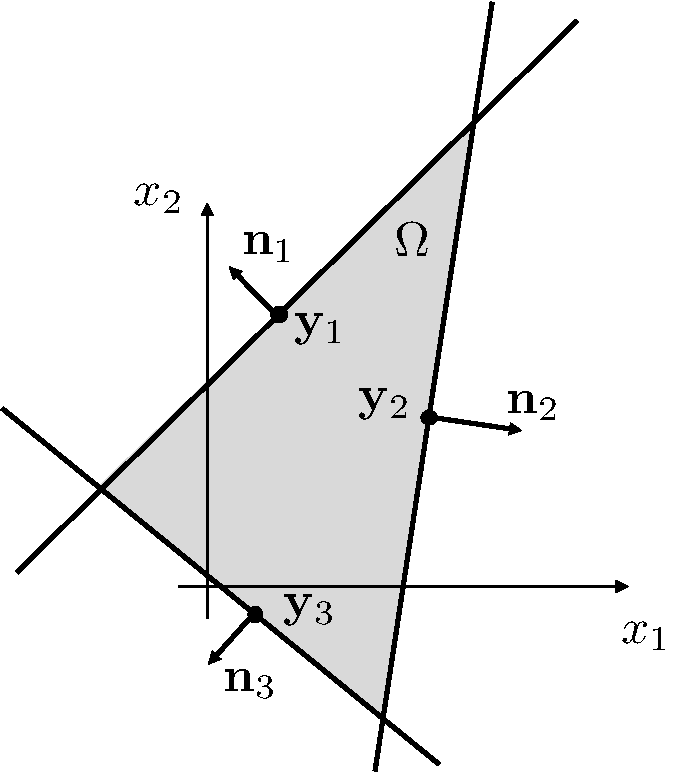
\includegraphics[width=0.5\textwidth]
						{figures/chap18_inequality_constraints}
				\end{center}
			\end{column}
		\end{columns}
		Where $\nbf_i$ is a vector normal to the linear constraint.	
	\end{example}
\end{frame}

%----------------------------------
\begin{frame}\frametitle{Constrained Optimization}
	A general constrained optimization problem can be written as
	\begin{mini*}|s|
		{x\in\Omega}{f(x)}{}{}
		\addConstraint{h_1(x)=0}
		\addConstraint{\vdots}
		\addConstraint{h_m(x)=0}
		\addConstraint{g_1(x)\leq 0}		
		\addConstraint{\vdots}
		\addConstraint{g_p(x)\leq 0}
	\end{mini*}
\end{frame}

%----------------------------------
\begin{frame}\frametitle{Constrained Optimization}
	Letting 
		\begin{align*}
			\hbf &= (h_1 \ldots h_m)^\top \\
			\gbf &= (g_1 \ldots g_p)^\top,		
		\end{align*}
 	we have
	\begin{mini*}|s|
		{x\in\Omega}{f(x)}{}{}
		\addConstraint{\hbf(x)=0}
		\addConstraint{\gbf(x)\leq 0}		
	\end{mini*} 	
	
	Equality constraints are easier to deal with than inequality constraints.
	
	\vfill
	
	We will first treat equality constraints, then inequality constraints.
	
\end{frame}


\end{document}